%% LaTeX2e class for student theses
%% thesis.tex
%% 
%% Karlsruhe Institute of Technology
%% Institute for Program Structures and Data Organization
%% Chair for Software Design and Quality (SDQ)
%%
%% Dr.-Ing. Erik Burger
%% burger@kit.edu
%%
%% Version 1.3.2, 2017-08-01

%% Available page modes: oneside, twoside
%% Available languages: english, ngerman
%% Available modes: draft, final (see README)
\documentclass[twoside, english]{sdqthesis}
\usepackage{mathtools}
\usepackage{pgfplots}
\pgfplotsset
{
	compat                   = newest,
	every tick/.append style = thin,
	width= .95 \textwidth
}

%% ---------------------------------
%% | Information about the thesis  |
%% ---------------------------------

%% Name of the author
\author{Emanuel Jöbstl}

%% Title (and possibly subtitle) of the thesis
\title{Reverberation robust acoustic modelling using time delay neural networks}

%% Type of the thesis 
\thesistype{Master's Thesis}

%% Change the institute here, ``IPD'' is default
\myinstitute{Interactive Systems Lab}

%% You can put a logo in the ``logos'' directory and include it here
%% instead of the SDQ logo
% \grouplogo{myfile}
%% Alternatively, you can disable the group logo
% TODO: Put the CMU logo in the logos directory, remove nogrouplogo
\nogrouplogo

%% The reviewers are the professors that grade your thesis
\reviewerone{Prof. A}
\reviewertwo{Prof. B}

%% The advisors are PhDs or Postdocs
\advisorone{M.Sc. C}
%% The second advisor can be omitted
\advisortwo{M.Sc. D}

%% Please enter the start end end time of your thesis
\editingtime{4. November 2017}{4. May 2018}

\settitle

%% --------------------------------
%% | Settings for word separation |
%% --------------------------------

%% Describe separation hints here.
%% For more details, see 
%% http://en.wikibooks.org/wiki/LaTeX/Text_Formatting#Hyphenation
\hyphenation{
% me-ta-mo-del
}

%% --------------------------------
%% | Bibliography                 |
%% --------------------------------

%% Use biber instead of BibTeX, see README
\usepackage[citestyle=numeric,style=numeric,backend=biber]{biblatex}
\addbibresource{thesis.bib}

%% ====================================
%% ====================================
%% ||                                ||
%% || Beginning of the main document ||
%% ||                                ||
%% ====================================
%% ====================================
\begin{document}

%% Set PDF metadata
\setpdf

%% Set the title
\maketitle

%% The Preamble begins here
\frontmatter

%% LaTeX2e class for student theses: Declaration of independent work
%% sections/declaration.tex
%% 
%% Karlsruhe Institute of Technology
%% Institute for Program Structures and Data Organization
%% Chair for Software Design and Quality (SDQ)
%%
%% Dr.-Ing. Erik Burger
%% burger@kit.edu
%%
%% Version 1.3.2, 2017-08-01

\thispagestyle{empty}
\null\vfill
\noindent\hbox to \textwidth{\hrulefill} 
\iflanguage{english}{I declare that I have developed and written the enclosed
thesis completely by myself, and have not used sources or means without
declaration in the text.}%
{Ich versichere wahrheitsgemäß, die Arbeit
selbstständig angefertigt, alle benutzten Hilfsmittel vollständig und genau
angegeben und alles kenntlich gemacht zu haben, was aus Arbeiten anderer
unverändert oder mit Änderungen entnommen wurde.}
 
 
%% ---------------------------------------------
%% | Replace PLACE and DATE with actual values |
%% ---------------------------------------------
\textbf{Pittsburgh, 1st of Mai, 2018}
\vspace{1.5cm}
 
\dotfill\hspace*{8.0cm}\\
\hspace*{2cm}(\theauthor) 
\cleardoublepage

\setcounter{page}{1}
\pagenumbering{roman}

%% ----------------
%% |   Abstract   |
%% ----------------
 
%% For theses written in English, an abstract both in English
%% and German is mandatory.
%%
%% For theses written in German, a German abstract is sufficient.
%%
%% The text is included from the following files:
%% - sections/abstract

\includeabstract

%% ------------------------
%% |   Table of Contents  |
%% ------------------------
\tableofcontents

\listoffigures
\listoftables

%% -----------------
%% |   Main part   |
%% -----------------

\mainmatter

%% LaTeX2e class for student theses
%% sections/content.tex
%% 
%% Karlsruhe Institute of Technology
%% Institute for Program Structures and Data Organization
%% Chair for Software Design and Quality (SDQ)
%%
%% Dr.-Ing. Erik Burger
%% burger@kit.edu
%%
%% Version 1.3.2, 2017-08-01

\chapter{Introduction}
\label{ch:Introduction}

Automated Speech Recognition is an important way of human computer interaction. The fundamental problem Automated Speech Recognition attempts to solve is to transform natural spoken language to text, which can then easily be processed by computer systems. Especially with the advent of smart mobile devices, more and more use cases for Automated Speech Recognition are available, mainly in the form of smart assistants as described in \cite{lopez2017alexa}. There are also many use cases which are not facing end users, for example the automated transcription of university lectures, as outlined in \cite{muller2016lecture}.

Despite the recent success of automated speech recognition, many systems still rely on microphones which are close to the speaker, or microphone arrays and beamforming. For many use cases, this is a serious draw back. Users might want to use their smart assistant without picking up their device every time. During lectures, it is hard to transcribe questions from the audience. 

\cite{yoshioka2012making} gives a good overview about the problems that arise when distant microphones are used. The most prominent problem is reverberation. Reverberation happens, informally speaking, when a signal is overlayed with weaker, delayed copies of itself. 

The goal of this work is to investiage how Automated Speech Recognition could be made more robust against reveberation. More specifically, a the focus is put on providing a more robust acoustic model using Time Delay Neural Networks. 

\section{Reveberation and reverbed Audio}

This section will focus on a formal definition of reverberation and provide some intuition why reveberation makes Automated Speech Recognition difficult. First, we give a very brief introduction to signal processing and system theory, according to the book \cite{leon2015signale}.

\subsection{Continous Signals and Systems}

An audio signal can, as any other continous \textit{signal}, be described as a continous function $y(t)$ where $t$ indicates the time. In literature, the argument $t$ is often dropped  when not explicitely needed to make equations easier to read.  
Signals can be fed into \textit{systems}, which in turn creates an output signal. In the context of this work, we only consider linear, time invariant systems. 
\\
Let $S$ be a linear time invariant system, $y_1$, $y_2$ continous signals, and $c_1$, $c_2$ constants. The following properties hold if and only if a given system is an linear time invariant system: 

\[S\{c_1 y_1(t) + c_2 y_2(t)\} = c_1 S\{y_1(t)\} + c_2 S\{y_2(t)\} \tag{linearity}\]

The linear property allows us to treat application of a system to a signal as a linear transformation in the function space our signals are defined in. 

\[y_1(t) = S\{y_2(t)\} \implies y_1(t - t0) = S\{y_2(t - t0)\} \tag{time invariance}\]

The time invariance propery guarantees that the behavior of a system never depends on the time. In other words, if the input signal to a system is shifted in time, the only difference to the output is a shift in time as well.

\[
\begin{rcases*}
y_1(t') = y_2(t') \\
x_1(t') = S\{y_1(t')\} \\ 
x_2(t') = S\{y_2(t')\} \\
\end{rcases*} \implies x_1(t') = x_2(t') \tag{causality}\]

The causality property guarantees that, if two signals are equal for all times $t'$ before a chosen time $t_0$, the output signals of the system processing this signals will also be equal up to this point. Simply put, the output of a system up to time $t_0$ can not depend on any input that happens after $t_0$. It is worth to note that all real systems are always causal. 
\\ \\
A linear time-invariant system can be characterized by its so called impulse response $g$, defined as the system output when presented with a so called dirac impulse $\delta$.

\[g(t) = S\{\delta(t)\}\]

The dirac impulse $\delta$ is a function that is formally defined by the following equation. 

\begin{align}
g(t_2) = \int_{-\infty}^{\infty} y(t)\delta(t - t_2) dt \label{eq:dirac} 
\end{align}

It can be said that the dirac impulse is zero for all $t$ not equal to zero. The integral over the dirac impulse defined to be one. 
\\ \\
Given definition \ref{eq:dirac}, as well as the linear property, we can show that the impulse response of a system is indeed sufficient to calculate the output signal for any given input signal. 
\begin{align*}
x(t) &= S\{y(t)\} \\
	 &= S\left\{\int_{-\infty}^{\infty} y(\tau)\delta(\tau - t) d\tau \right\} \\
	 &= \int_{-\infty}^{\infty} y(\tau)S\{\delta(\tau - t)\} d\tau \\
	 &= \int_{-\infty}^{\infty} y(\tau)g(\tau - t) d\tau
\end{align*}

Furthermore, we define the convolution operation, $*$, for two given signals as follows.

\[
 (y_1 * y_2)(t) = \int_{-\infty}^{\infty} y(\tau)y_2(\tau - t) d\tau \tag{(convolution)}
\]

A convolution is thus an operation that combines two functions to create a new function. Given this definition, we can write the output signal $x$ of a system $S$ given an input signal $y$ as convolution with the impulse response $g$ of the system. 

\[
x(t) = S\{y(t)\} = (y * g)(t)
\]

\subsection{Properties of Reverberation}

The acoustic properties of a room can be approximated as a linear time invariant system. The properties of this system are dependent on the properties of the room itself, for example the shape, size and surface of the wall, as well as the location of the sound source and the location of the receiver. Especially regarding automated speech recognition, \cite{ritter2016training} gives results that show that the location of a speaker relative to the microphone can have a very large impact on recognition results.

The measured impulse response of a real reveberation can be seen in figure \ref{fig:air_rir}. This specific sample is taken from the Aachen Impulse Response database \cite{jeub2009binaural}. Such a sample can be created by creating a very brief sound impulse, for example a clap, in an otherwise silent room, and then recording the sound for a few seconds. 

As described in \cite{yoshioka2012making}, we can divide the impulse response into the direct sound itself, early reflections, and late reverberation. The intuition behind is that the original sound wave arrives at the receiver first. After that, reflections of the signal which were reflected once by the walls of the room arrive. These reflections are already dampened significantly. Then, reflections of reflections will be received, and so on, until the sound waves become so weak that the room is silent again. 
\\ \\
\begin{minipage}{\linewidth}
	\makebox[\linewidth]{
		\begin{tikzpicture}
			\begin{axis}[ytick=\empty,height=6cm, ylabel=Amplitude, xlabel=Milliseconds, 
			xticklabel style={name=T\ticknum}]
			\addplot table [x expr=\coordindex / 4,y=amplitude,color=black,mark=none] {data/air0053bilecture};
			
			\end{axis}	
			\draw[] (1.2,4) -- (1,4) node[anchor=east,font=\tiny] {Sound};
			\draw[decorate, decoration={brace}] (1.3,3.2) -- (3.00,3.2) node[midway, anchor=south,font=\tiny] {Early Reflections};	
			\draw[decorate, decoration={brace}] (3.05,3.2) -- (11.8,3.2) node[midway, anchor=south,font=\tiny] {Late Reverberations};	
			\label{fig:air_rir}
		\end{tikzpicture}
	}
	\captionof{figure}{Room impulse response of a lecture hall}
\end{minipage}

It is important to note that late reveberations can be measureable for several hundred milliseconds.\\\\

To illustrate the impact of reflection and reveberation in a more formal way, we can use the decomposition into direct sound, early reflection, and late reverberation. We define a rather crude approximation of a room impulse response that subsequently overlays an audio signal with weaker copies of itself.

\[
g_{rir}(t) = w_0 \delta(t) + \sum_{1}^{n} w_n * delta(t - t_n)
\]

Here, $w_n$ are weighting factors, which represent the dampening of our reflections. $t_n$ are the delays until our reflection is received. We now consider the system $S_{rir}$ associated with the impulse response $g_{rir}$, apply the audio signal $y$ and observe the output $x$.

\begin{align*}
x(t) &= S_{rir}\{y(t)\} \\
     &= (g_{rir} * y)(t) \\
     &= \int_{-\infty}^{\infty} g(\tau)y(\tau - t) d\tau \\
     &= \int_{-\infty}^{\infty} \left[ w_0 \delta(t) + \sum_{n} w_n * \delta(t - t_n)\right] y(\tau - t) d\tau \\
     &= \int_{-\infty}^{\infty} \delta(t) y(\tau - t) d\tau + \sum_{n}  \int_{-\infty}^{\infty} w_n \delta(t - t_n) y(\tau - t) d\tau  \\
     &= w_0 y(t) + \sum_{n} w_n y(t - t_n)
\end{align*}

If the room impulse response is non-zero over at a certain time interval $t_n$, the audio signal produced at $t$ will still influence the received signal $x$ at $t + t_n$. 

\subsection{Impact of Reverberation on Digital Audio Samples}

Before formally introducing automated speech recognition during a later chapter, we want to show that the impact of reverberation can be significant for many applications that process sound or speech.\\ \\
Before a signal can be processed on a computer, it has to be measured. This process is called \textit{sampling}. Formally, we can describe sampling as the following operation, where $t_A$ is called the sampling interval. We call $y_{digital}$ a discrete signal. 

\[
y_{digital}(t) = y(t) * \sum_{n = 0}^{\infty} \delta{t - nt_A} 
\]

Since this yields a time series of inifinite length, signals are usually cut into pieces, which are then independently processed from each other. This is called windowing. For the most simple form of windowing, we can set all signal values outside of a certain range to be zero. Formally, this can be defined by multiplying the signal with a rectangle function $\sigma_{rect,a}(t)$ .

\[
\sigma_{rect,a}(t) = \begin{cases}
1 &,-a < t < a \\
0
\end{cases}
\]

When working with signals, especially for classification tasks, methods built upon the \textit{fourier transform} are used very often. The fourier transform transforms a signal $y(t)$ from its time domain to the frequency domain $Y(f)$. The resulting function $Y(f)$ is called the spectrum and gives the distribution of energy over all frequencies for the original signal $y(t)$. The fourier transformation can be defined for continous or descrete signals, as well as for descrete and windowed signals. In the case of descrete and windowed signal, this is called the \textit{short time fourier transform}, which was first described in \cite{gabor1946theory}. It can formally be defined as follows, with an arbritary window function $\sigma$:

\[
Y(n, \omega) = \sum_{m = -\infty}^{\infty} y(mt_A) \sigma((n - m)t_A) e^{-j \omega n}  
\]

The function $Y(n, \omega)$ gives the energy for a certain time window $n$ and a frequency window $\omega$. The time resolution depends reciprocally on the frequency resolution and vice versa. It is not possible to increase the frequency resolution while not decreasing the time resolution.\\ \\

We can investigate the effects of a reverbed signal on the short time fourier transform by applying the same approach as in the previous chapter. The resulting short time fourier spectrum of the reverbed and sampled signal is given as follows.

\begin{align*}
Y(n, \omega) = \sum_{m = -\infty}^{\infty} w_0 y(mt_A) \sigma((n - m)t_A) e^{-j \omega n} + 
\sum_{m = -\infty}^{\infty} \sum_{n} w_n y(mt_A - t_n) \sigma((n - m)t_A) e^{-j \omega n}  
\label{eq:stftnoise}
\end{align*}

Equation \ref{eq:stftnoise} shows that, for large $t_n$ and $w_n$, significant noise is added to neighboring time windows. To recapitulate from the last chapter, the $t_n$ for a large room can be up to several tenths of seconds, while the window size for most applications is in the hundrets of milliseconds. 
\\ \\
This mathematic observation shall serve as a motivation for this work. Reverberation, especially late reverberation can be a hard problem that significantly distorts measurements of signals. We conclude the introduction with 

\begin{minipage}{\linewidth}
	\makebox[\linewidth]{
		\begin{tikzpicture}
		\begin{axis}[xlabel=Time, ylabel=Frequency, ytick=\empty, width= .50\textwidth]
		\addplot [] 
		graphics[xmin=0,xmax=3,ymin=0,ymax=1] {images/abc_spectrogram.png};
		\end{axis}
		\end{tikzpicture}
		\begin{tikzpicture}
		\begin{axis}[xlabel=Time, ylabel=\empty, ytick=\empty, width= .50\textwidth]
		\addplot [] 
		graphics[xmin=0,xmax=3,ymin=0,ymax=1] {images/abc_noise_spectrogram.png};
		\end{axis}
		\end{tikzpicture}
	}
	\captionof{figure}{Room impulse response of a lecture hall}
\end{minipage}

TODO: Nice picture of noisy STFT







\section{Related Work}
\label{ch:related_work}
This chapter will enumerate related work on acoustic modelling using TDNNs. 
%% LaTeX2e class for student theses
%% sections/content.tex
%% 
%% Karlsruhe Institute of Technology
%% Institute for Program Structures and Data Organization
%% Chair for Software Design and Quality (SDQ)
%%
%% Dr.-Ing. Erik Burger
%% burger@kit.edu
%%
%% Version 1.3.2, 2017-08-01

\chapter{Design of a TDNN acoustic model}
\label{ch:tdnn_design}
Our approach for creating a robust TDNN acoustic model is to find a TDNN model that performs good on clean data first. Therefore, we had to make several design decisions. Most of the design decisions were justified by experiments, while some were taken from related work. This chapter summarizes the decisions made and the corresponding results. It should be noted that the experiments about robust acoustic modeling with TDNNs described in \cite{peddinti2015jhu} and \cite{peddinti2015reverberation} provided the main motivation for this work, therefore we based some of our parameters on their result.
\section{Training Data and System Setup}
All experiments in this work only concern the neural network part of our acoustic model, which is a HMM/TDNN hybrid. The speech recognition system itself, as well as all data, the HMM part of the acoustic model, the dictionary and the language model, are based upon the system described in \cite{nguyen20162016}. The system is built upon the Janus recognition toolkit \cite{finke1997karlsruhe}. We utilize a four-gram language model and the CMU Pronouncing Dictionary \cite{cmudict}, which uses 39 phones. The acoustic model uses quinphones and has 8156 different distributions, which means that the HMM part of our acoustic model has 8156 different states. \\ \\
The training and test dataset for the acoustic model consist of 468 hours of English speech from the TED-LIUM v2 \cite{rousseau2014enhancing}, Broadcast News \cite{graff19971996} and Quaero 2010-2012 datasets. From these 468~hours, 17~hours are randomly selected as test set, 451~hours are used for the training set. \\ \\
The development dataset, used for tuning the decoder parameters, consists of the english IWSLT 2013 evaluation dataset for the ASR track \cite{cettolo2013report}. This dataset consists of 3.9~hours of TED talks. The word error rates for all experiments in this chapter were measured on this development set. \\ \\ 
Each frame of samples in the datasets consists of 40~log-mel features which were normalized over the whole utterance to have mean zero and variance two. Each frame covers 32~milliseconds. The frame shift between successive frames is 10~milliseconds. The sampling rate of the audio data was 16~kHz. \\ \\
The neural network training was done using a custom framework, build on top of PyTorch \cite{paszke2017automatic}. Pytorch is a machine learning framework that supports GPU accelleration, parallelization along multiple systems and automatic differentiation. In the context of this work, several contributions were made to the PyTorch framework.  
\section{Neural Network Parameters}
This section focuses on parameters that are related to the neural network design. For all models in this section, the word error rate was estimated by using $l_p$ and $l_z$ that were tuned for each model separately. The priors were estimated by counting labels over the whole training set.
\subsection{Input Context}
The time input context of all our TDNN models is $(-13,9)$, which means the TDNN sees the current frame, thirteen frames in the past, and nine frames in the future. This parameter was taken from the smallest TDNN model described in \cite{peddinti2015reverberation}.
\subsection{Count and Width of Layers}
The count of layers and width of each layer is one of the most important design parameters for neural networks. As in \cite{peddinti2015reverberation}, all our models use the same amount of channels for each TDNN layer. Only the count of observed time frames changes with each layer. \\ \\
\begin{minipage}{\linewidth}
	\centering
	\begin{tabular}{@{\extracolsep{4pt}}lccccccccc@{}}
		\toprule
		Model:      & \multicolumn{4}{c}{Four Layer}       & \multicolumn{5}{c}{Five Layer}\\\cmidrule[1pt]{1-1}\cmidrule[1pt]{2-5}\cmidrule[1pt]{6-10}
		Layer       & 1 & 2 & 3 & 4    & 1 & 2 & 3 & 4 & 5 \\\cmidrule{2-5}\cmidrule{6-10}
		Kernel Size & 5 & 2 & 2 & 2    & 5 & 5 & 3 & 2 & 2 \\
		Stride      & 3 & 2 & 2 & 2    & 2 & 1 & 1 & 1 & 1 \\
		\bottomrule
	\end{tabular}
	\captionof{table}{Kernel size and stride parameters for the two different architectures}
	\label{tbl:tdnn_layer_design}
\end{minipage} \\ \\
We decided to test a four layer model with exactly the same parameters as the smallest model in \cite{peddinti2015reverberation}. This model also included a splicing layer after layer one. The splicing configuration was $(0, 1, 2, 3, 3, 4, 5, 6)$, relative to the previous layer. For the second model we tested, we decided to use larger kernels and one more layer. For this purpose, we removed the splicing layer and increased the layer count to five. Table \ref{tbl:tdnn_layer_design} gives the kernel size and stride over time for each layer in each architecture. For both models, we used an L2 pooling nonlinearity with group size of ten followed by a batch normalization layer after each TDNN layer.
\\
Figure \ref{fig:tdnn_layer_design} shows the word error rate for the two different architectures, given the count of channels. It can be seen that the four-layer architecture performed better than the five-layer architecture. We found the optimal count of channels  for the four-layer model to be 300. This contradicts \cite{peddinti2015reverberation}, where 400 channels were used. \\ \\
\begin{minipage}{\linewidth}
	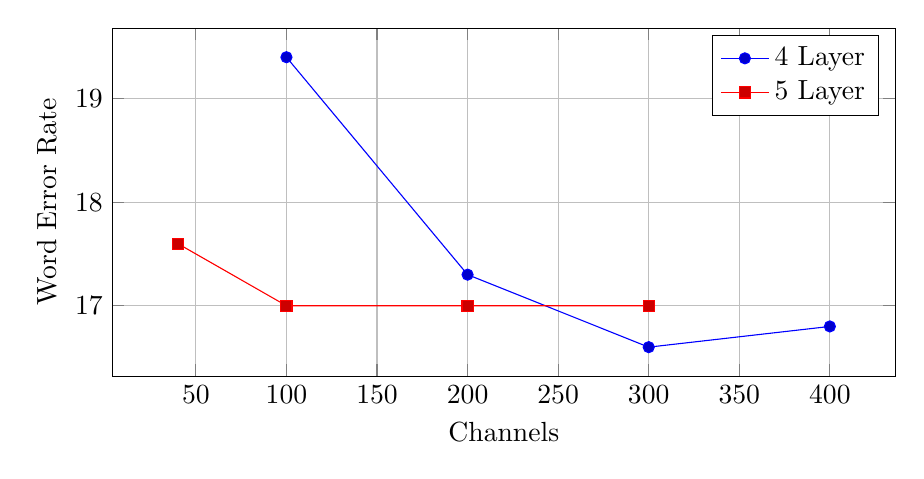
\begin{tikzpicture}
	\begin{axis}[ylabel=Word Error Rate, xlabel=Channels, height=6cm, 
	xticklabel style={name=T\ticknum},grid=major]
	\addplot coordinates {
		(100,19.4) %994
		(200,17.3) %999
		(300,16.6) %1009
		(400,16.8) %1010
	};
	\addlegendentry{4 Layer};
	\addplot coordinates {
		(40,17.6) %1040
		(100,17.0) %i3
		(200,17.0) %1039
		(300,17.0) %1036
	};
	\addlegendentry{5 Layer};
	\end{axis}
	\end{tikzpicture}
	\captionof{figure}{Word Error Rate for different choices of layer and channel count}
	\label{fig:tdnn_layer_design}
\end{minipage} 
\subsection{Nonlinearity}
\label{sec:tdnn_nonlin}
Following \cite{zhang2014improving}, we tested L2 pooling nonlinearity with group size if ten after each TDNN layer. Using the L2 norm can be problematic, as the gradient is not defined when all inputs in the pooling group are zero. The authors of \cite{zhang2014improving} propose to use a modified batch normalization layer after each LP-pooling layer, which solves the problem. We propose an alternate approach, which is setting the gradient to zero if all inputs become zero. Furthermore, we also tested max pooling as a possible nonlinearity. All experiments were conducted on the four-layer architecture described before. Figure \ref{fig:tdnn_nonlinearity} shows the results. \\ \\
\begin{minipage}{\linewidth}
	\centering
	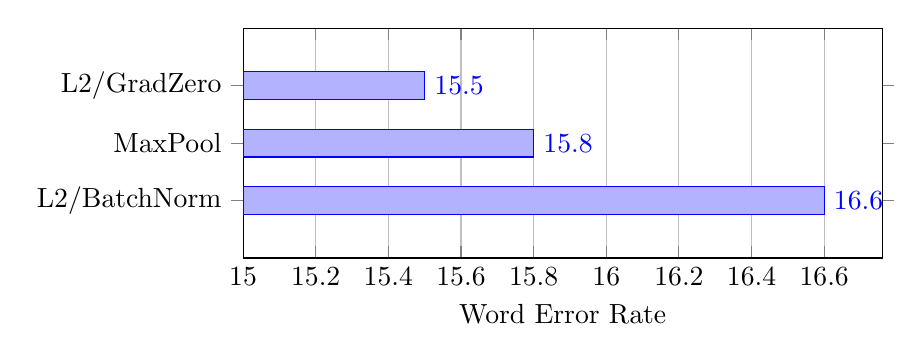
\begin{tikzpicture}
		\begin{axis}[
		xbar,xmajorgrids=true,
		width=0.8\linewidth,height=4.5cm, enlarge y limits=0.5,
		xmin=15,xlabel={Word Error Rate},
		symbolic y coords={L2/BatchNorm,MaxPool,L2/GradZero},
		ytick=data,nodes near coords, nodes near coords align={horizontal},
		]
		%1009, I24, I12
		% All with only l[/lz/mb tuning, no custom priors and no softmax
		\addplot coordinates {(15.5,L2/GradZero) (15.8,MaxPool) 
		(16.6,L2/BatchNorm)};
		\end{axis}
	\end{tikzpicture}
	\captionof{figure}{Word Error Rate for different choices of nonlinearities}
	\label{fig:tdnn_nonlinearity}
\end{minipage} \\ \\
In our case, the usage of L2 pooling with a modified gradient outperformed the other nonlinearities. It was not possible to compare L2 pooling without any modifications, as our training became unstable. 
\section{Training Setup}
This section is focused on the training setup for our acoustic model. Out setup is closely related to the setup described in \cite{nguyen20162016}. We essentially use the same speech recognition system, the same labels, as well as the same samples for training our acoustic model.
\subsection{Shuffling and Preparation of Dataset}
For our experiments, we benchmarked different shuffling strategies with a six-layer fully connected network. Shuffling of the whole dataset once before training, and shuffling of the whole dataset before each epoch. The results can be seen in figure \ref{fig:tdnn_shuffling}. \\ \\
\begin{minipage}{\linewidth}
	\centering
	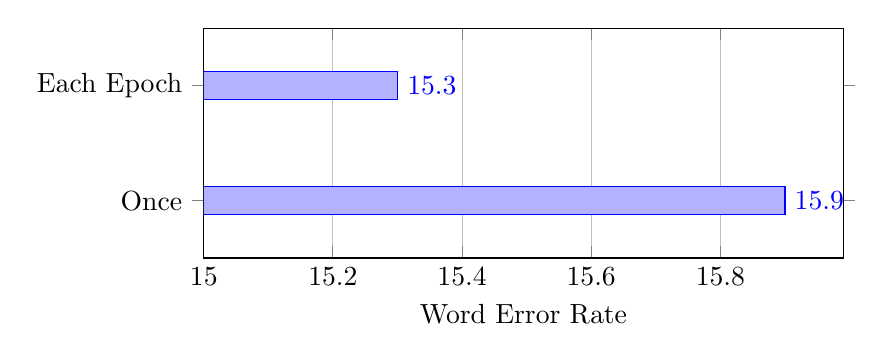
\begin{tikzpicture}
	\begin{axis}[
	xbar,xmajorgrids=true,
	width=0.8\linewidth,height=4.5cm, enlarge y limits=0.5,
	xmin=15,xlabel={Word Error Rate},
	symbolic y coords={Once,Each Epoch},
	ytick=data,nodes near coords, nodes near coords align={horizontal},
	]
	\addplot coordinates {(15.9,Once) (15.3,Each Epoch)};
	\end{axis}
	\end{tikzpicture}
	\captionof{figure}{Word Error Rate for different shuffling strategies}
	\label{fig:tdnn_shuffling}
\end{minipage} \\ \\
We can see that shuffling of the training dataset before each epoch decreased the word error rate. \\
\subsection{Learning Rate and Learning Rate Decay}
As in \cite{nguyen20162016}, we utilize the newbob learning rate scheduler for training for stochastic gradient descend, with an initial learning rate of $0.08$ and a momentum of $5$. The SGD variant used is the introduced in section \ref{sec:momentum}, as this was also used in \cite{nguyen20162016}\footnote{This SGD variant is not equal to the default SGD variant implemented in pytorch.}. Figure \ref{fig:newbob_wer} shows the word error rate per epoch when using newbob. It can be seen that there were almost no improvements during epoch four, but the word error rate improved as soon as the decaying started after epoch four. Figure \ref{fig:newbob_fer} shows the frame error rate per epoch for the same training run. It can be seen that exponential decay reduces the frame error rate significantly. The model used for this experiment was the four layer TDNN introduced in the previous section.
\\ \\
\begin{minipage}{\linewidth}
	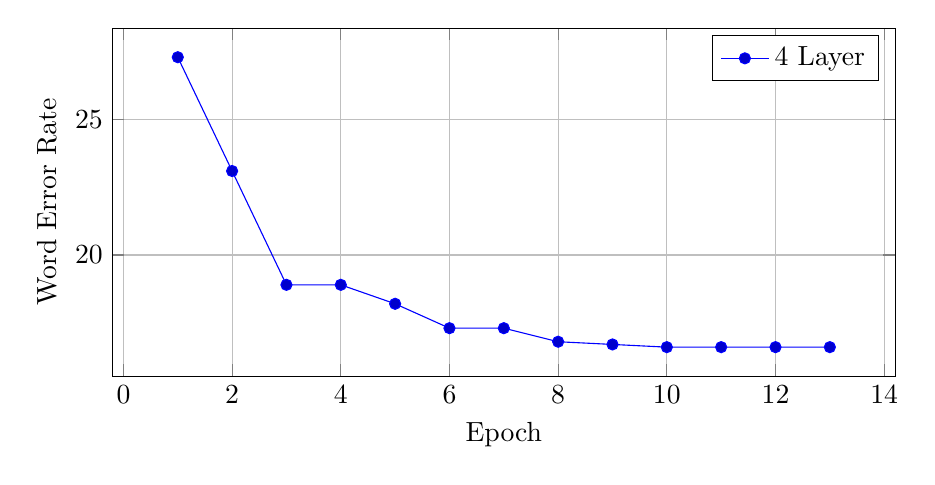
\begin{tikzpicture}
	\begin{axis}[ylabel=Word Error Rate, xlabel=Epoch, height=6cm, 
	xticklabel style={name=T\ticknum},grid=major]
	% I12
	\addplot coordinates {
		(1,27.3)
		(2,23.1)
		(3,18.9)
		(4,18.9)
		(5,18.2)
		(6,17.3)
		(7,17.3)
		(8,16.8)		
		(9,16.7)
		(10,16.6)
		(11,16.6)
		(12,16.6)
		(13,16.6)
	};
	\addlegendentry{4 Layer};
	\end{axis}
	\end{tikzpicture}
	\captionof{figure}{Word Error Rate per Epoch when using newbob training. The exponential decaying of the learning rate started after epoch four.}
	\label{fig:newbob_wer}
\end{minipage}
 \\ \\
\begin{minipage}{\linewidth}
	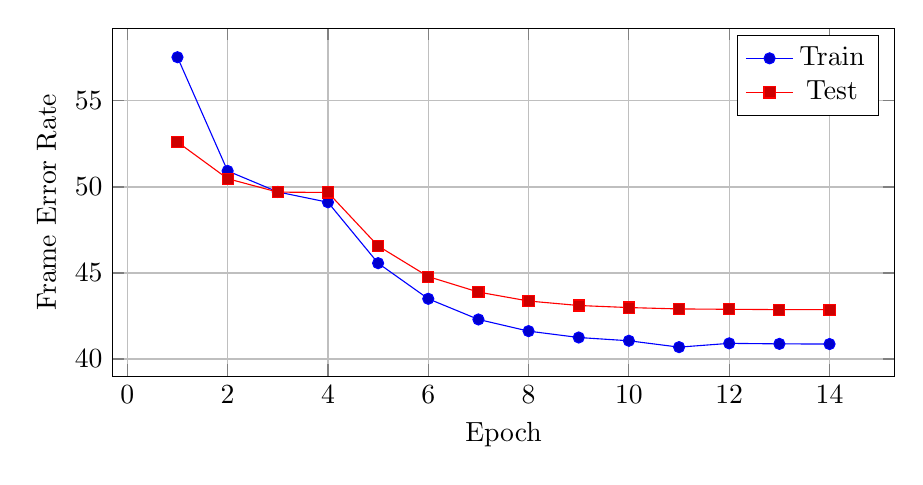
\begin{tikzpicture}
	\begin{axis}[ylabel=Frame Error Rate, xlabel=Epoch, height=6cm, 
	xticklabel style={name=T\ticknum},grid=major]
	%I12
	\addplot coordinates {
		(1,57.54)
		(2,50.93)
		(3,49.71)
		(4,49.11)
		(5,45.57)
		(6,43.50)
		(7,42.30)
		(8,41.62)		
		(9,41.25)
		(10,41.06)
		(11,40.69)
		(12,40.91)
		(13,40.88)
		(14,40.87)
	};
	\addlegendentry{Train};
	\addplot coordinates {
		(1,52.61)
		(2,50.48)
		(3,49.70)
		(4,49.68)
		(5,46.57)
		(6,44.79)
		(7,43.89)
		(8,43.37)		
		(9,43.11)
		(10,42.99)
		(11,42.91)
		(12,42.89)
		(13,42.87)
		(14,42.87)
	};
	\addlegendentry{Test};
	\end{axis}
	\end{tikzpicture}
	\captionof{figure}{Frame Error Rate per Epoch when using newbob training. The exponential decaying of the learning rate started after epoch four.}
	\label{fig:newbob_fer}
\end{minipage}
\subsection{MMIE Training}
Since the experiments described in \cite{peddinti2015jhu} show improvement when sMBR discriminative training is used, we attempted to use discriminative based training as well. Our implementation used maximum mutual information estimation, as described in section \ref{sec:mmie}. We picked this training variant as a first step, since it is easier to implement than any variant of overall risk criterion estimation. Both approaches should show some improvement over cross entropy loss on frame level, according to several bodies of work \cite{povey2005discriminative} \cite{ghoshal2013sequence}. \\ \\
For MMIE training, we pre-trained a four layer TDNN acoustic model with frame-based cross entropy loss for a single epoch. Then, we started MMIE training on a per-utterance basis. For this purpose, we wrote a module that enabled interoperability between the Janus recognition toolkit and PyTorch. The training was done on multiple machines with a total of 256 processors, the gradients were averaged before each SGD step. \\ \\
While our experiments consistently showed high improvements in terms of frame error rate, the word error rate increased significantly: The model reached a WER of $17.6$ using cross entropy loss, but only a WER $25.6$ was reached after the MMIE training finished the first epoch. This effect was also described in more practically oriented literature \cite{su2013error} for MMIE without any further modifications. 

\begin{minipage}{\linewidth}
	\begin{minipage}{0.5\linewidth}
	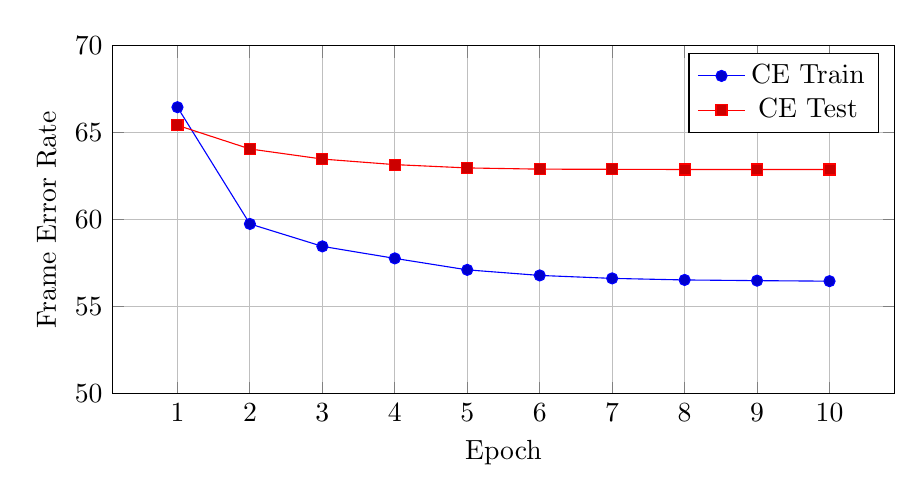
\begin{tikzpicture}
	\begin{axis}[ylabel=Frame Error Rate, xlabel=Epoch, height=6cm, 
	ymin=50, ymax=70,
	xticklabel style={name=T\ticknum},grid=major]
	%1040
	\addplot coordinates {
		(1,66.47)
		(2,59.76)
		(3,58.47)
		(4,57.78)
		(5,57.12)
		(6,56.80)
		(7,56.63)
		(8,56.54)		
		(9,56.50)
		(10,56.47)
	};
	\addlegendentry{CE Train};
	\addplot coordinates {
		(1,65.43)
		(2,64.07)
		(3,63.49)
		(4,63.17)
		(5,62.98)
		(6,62.91)
		(7,62.90)
		(8,62.89)		
		(9,62.89)
		(10,62.89)
	};
	\addlegendentry{CE Test};
	\end{axis}
	\end{tikzpicture}
\end{minipage}
\hfill
\begin{minipage}{0.5\linewidth}
	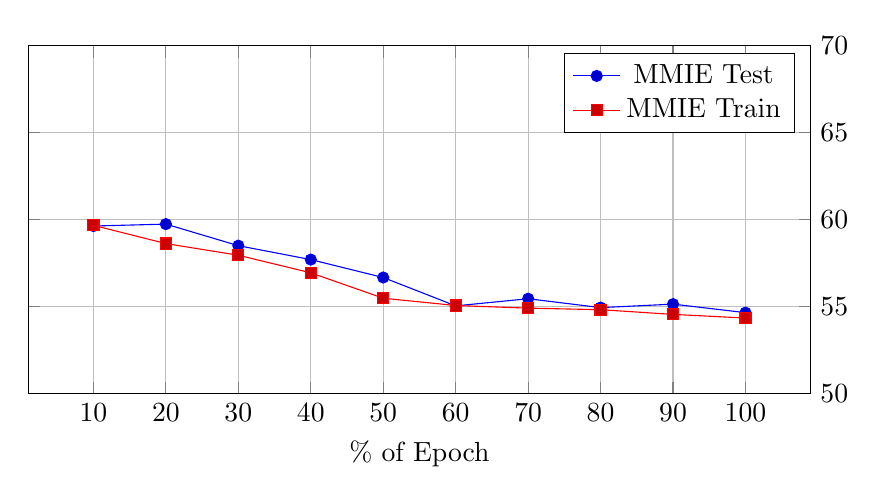
\begin{tikzpicture}
	\begin{axis}[xlabel=\% of Epoch, height=6cm, 
	 ylabel near ticks, yticklabel pos=right,
	ymin=50, ymax=70,
	xticklabel style={name=T\ticknum},grid=major]
	%1040 SMBR 24
	\addplot coordinates {
		(10,59.64)
		(20,59.75)
		(30,58.51)
		(40,57.71)
		(50,56.68)
		(60,55.05)
		(70,55.46)
		(80,54.95)		
		(90,55.15)
		(100,54.66)
	};
	\addlegendentry{MMIE Test};
	\addplot coordinates {
		(10,59.68)
		(20,58.631)
		(30,57.96)
		(40,56.95)
		(50,55.49)
		(60,55.07)
		(70,54.92)
		(80,54.83)		
		(90,54.56)
		(100,54.35)
	};
	\addlegendentry{MMIE Train};
	\end{axis}
	\end{tikzpicture}
\end{minipage}
	\captionof{figure}{Frame Error Rate per Epoch when using cross entropy loss, as well as Frame Error Rate over a single epoch when using MMIE on a TDNN}
	\label{fig:mmie_fer}
\end{minipage} \\ \\
Detailed results regarding the frame error rate are shown in figure \ref{fig:mmie_fer}. It can be seen that the MMIE training converged significantly faster than cross entropy training. Also, the error on the test data set is significantly closer to the error on the training data set. 
\iffalse
% This is the training for a Fully Connected net with ReLU, which diverged. There are examples in the litherature which did NOT diverge. 
\begin{minipage}{\linewidth}
	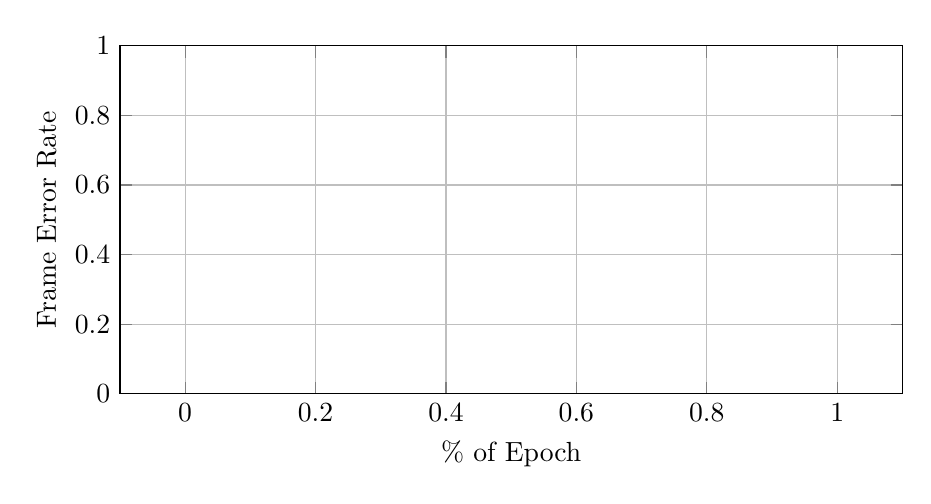
\begin{tikzpicture}
	\begin{axis}[ylabel=Frame Error Rate, xlabel=\% of Epoch, height=6cm, 
	ymin=50, ymax=70,
	xticklabel style={name=T\ticknum},grid=major]
	%1040
	\addplot coordinates {
		(10,75.2618)
		(20,75.2638)
		(30,75.2839)
		(40,76.25)
		(50,76.99539216)
		(60,87.03598039)
		(70,83.21137255)
		(80, 84.23852941)
	};
	\addlegendentry{MMIE Train};
	\end{axis}
	\end{tikzpicture}
	\label{fig:mmie_fer_fc}
\end{minipage}
\fi
\\ These results were achieved using the four-layer TDNN model. Caution has to be taken when interpreting the results: While the amount of data in both test data sets is the same, they are not equal as training and testing for MMIE happens on per-utterance basis, while the test and training sets for the cross entropy loss based training were created on per-frame basis. \\ \\
Although the results regarding frame error rate look interesting, we did not pursue this approach any further, due to the resulting high word-error rates and the numerous details one has to consider for working MMIE training on neural networks \cite{su2013error}.

\section{Decoding Parameters}
Tuning decoding parameters is important for good achieving a high accuracy on word level. The decoding parameters are not directly related to the acoustic model, but rather the decoding process. Different acoustic models might still require different decoding parameters for best performance. 
\subsection{Acoustic Model Scaling and Length Penalty}
Our experiments have shown that the $l_p$ and $l_z$ parameters are depending on each other. Therefore we can not optimize them separately. We choose to perform a grid search over a reasonable parameter space. \\ \\
\begin{minipage}{\linewidth}
\centering
\begin{tikzpicture}
\begin{axis}[grid=both,zlabel=Word Error Rate,xlabel=$l_p$,ylabel=$l_z$,width=0.7\linewidth]
	\addplot3[surf,mesh/cols=10,z buffer=sort] file {data/lp_lz_i12};
\end{axis}
\end{tikzpicture}
\captionof{figure}{Illustrative example of the word error rate for different $l_p$ and $l_z$ parameters for a four-layer TDNN}
\label{fig:lp_lz}
\end{minipage}
\\ \\
An example impact of the $l_p$ and $l_z$ for two different models are illustrated in figure \ref{fig:lp_lz}. Our experiments have shown that the optimal parameters are similar for each of the models we tested. It is still advisable to fine tune the parameters for each model. Taking the initial values for the grid search from an similar model usually leads to good results.
\subsection{Master Beam}
We tested several architectures with different master beams. Master beams between four and six appeared to work best, but we did not find any pattern that correlated with the network architecture. This indicates that the optimal master beam depends on several factors, not just on the architecture of the neural network model itself. 
\subsection{Neural Network Priors}
\label{sec:tdnn_prior}
As described in section \ref{sec:ce_loss}, it is important to scale the posteriors generated by the neural network with priors. We tested two different approaches of generating the priors: Generating them from the complete test dataset and also generating them from the output of a trained model. In the second case, we selected thirty minutes of speech data randomly from our dataset, computed the neural network output on it, and counted the occurrence of each label in the output. \\ \\
\begin{minipage}{\linewidth}
	\centering
	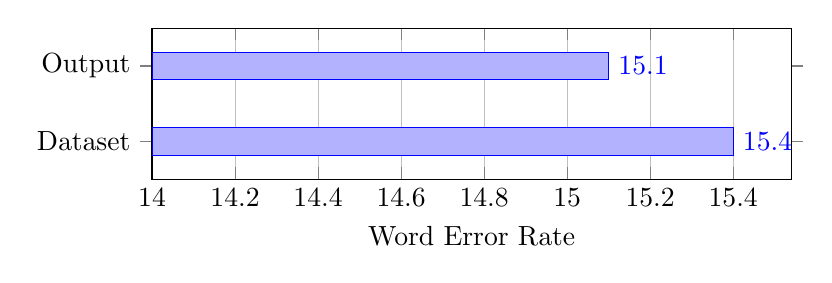
\begin{tikzpicture}
	\begin{axis}[
	xbar,xmajorgrids=true,
	width=0.8\linewidth,height=3.5cm, enlarge y limits=0.5,
	xmin=14,xlabel={Word Error Rate},
	symbolic y coords={Dataset,Output},
	ytick=data,nodes near coords, nodes near coords align={horizontal},
	]
	\addplot coordinates {(15.4,Dataset) (15.1,Output)};
	\end{axis}
	\end{tikzpicture}
	\captionof{figure}{Word Error Rate for priors estimated from the dataset and the model output}
	\label{fig:wer_priors}
\end{minipage} 
\\
As illustrated in figure \ref{fig:wer_priors}, calculating the priors from the the output of the model decreased the word error rate significantly. These experiments were done on the four-layered TDNN model. 
\subsection{Softmax Smoothing}
We also tested the impact of softmax smoothing on the neural network output. The motivation is that a beam search through a hidden Markov model does not work very well when the acoustic model is overconfident regarding certain states. Figure \ref{fig:softmax_fer} shows that softmax smoothing decreased the word error rate for our four-layer TDNN model. \\ \\
\begin{minipage}{\linewidth}
	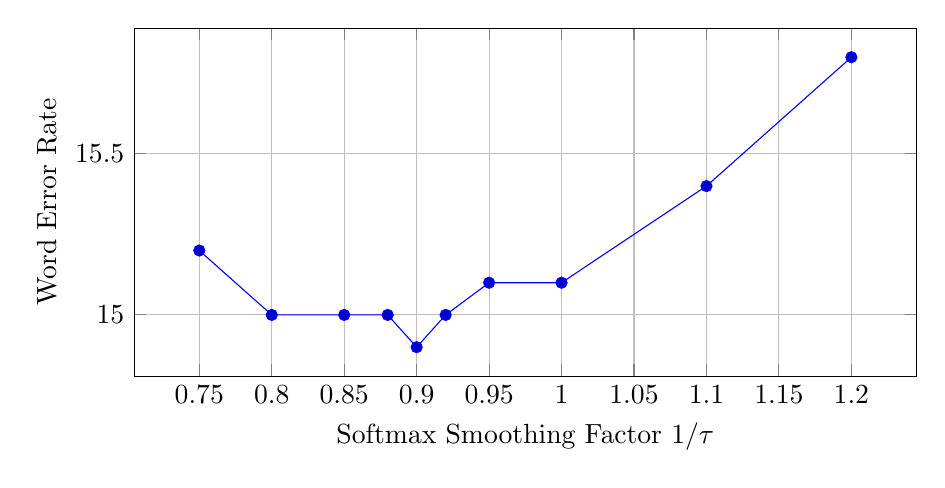
\begin{tikzpicture}
	\begin{axis}[ylabel=Word Error Rate, xlabel=Softmax Smoothing Factor $1/\tau$, height=6cm, 
	xticklabel style={name=T\ticknum},grid=major]
	%I12
	\addplot coordinates {
		(0.75,15.2)
		(0.8,15)
		(0.85,15)
		(0.88,15)
		(0.9,14.9)
		(0.92,15)
		(0.95,15.1)
		(1,15.1)
		(1.1,15.4)
		(1.2,15.8)
	};
	\end{axis}
	\end{tikzpicture}
	\captionof{figure}{Word Error Rate per softmax adjustment $1/\tau$ for a four-layer TDNN model}
	\label{fig:softmax_fer}
\end{minipage} \\ \\


\iffalse
\label{ch:approach}
This chapter describes our approach for acoustic modelling using TDNNs on a high level. 
We will also give a brief overview over unknown hyperparemters and design decisions,
as well as a coarse overview over the structure of our implementation. 

\chapter{Experiment Setup}
\label{ch:experiment_setup}
This chapter should describe the detailed preleminaries and hyperparemters of our training and evaluation setup:
\begin{itemize}
    \item which data, and which preprocessing was used
    \item how was the data reverbed
    \item which learning rate schedulers, optimizers, loss functions were used
    \item which mechanisms were used to make the training faster and scalable
\end{itemize}
\fi
%% LaTeX2e class for student theses
%% sections/evaluation.tex
%% 
%% Karlsruhe Institute of Technology
%% Institute for Program Structures and Data Organization
%% Chair for Software Design and Quality (SDQ)
%%
%% Dr.-Ing. Erik Burger
%% burger@kit.edu
%%
%% Version 1.3.2, 2017-08-01

\chapter{Evaluation on Reverberated Data}
\label{ch:results}
This section contains the final evaluation. It describes how different models performed on reverberated data.
\section{Neural Network Models}
We compare the four-layer TDNN model with a fully connected baseline model that was also used in \cite{nguyen20162016}. 
\subsection{TDNN Model}
The TDNN model, which can be seen in figure \ref{fig:final_tdnn} is based on the results found in chapter \ref{ch:tdnn_design}. \\ 
\begin{minipage}{\linewidth}
	\vspace{5mm}
	\begin{tikzpicture}[x=1.8cm, y=1.5cm]
	% Input layer
	\node[text width=3cm] at (-1,0) {Input ($23*40$)};
	\foreach \m in {2,3,...,22}
	\node [tdnn neuron] (input-\m) at (\m*0.25,0) {};
	
	\node [tdnn neuron, label=below:$x_{t - 13}$] (input-1) at (1*0.25,0) {};
	\node [tdnn neuron, label=below:$x_{t + 9}$] (input-23) at (23*0.25,0) {};
	
	% TDNN 1
	\node[text width=3cm] at (-1,0.5) {TDNN/LP 1};
	\node[text width=3cm] at (-1,1) {Hidden ($7*300$)};
	\foreach \m [count=\y] in {1,2,...,7}
	\node [tdnn neuron] (hidden-1-\m) at (\y*0.25*3,1) {};
	
	% Splice
	\node[text width=3cm] at (-1,1.5) {Splice};
	\node[text width=3cm] at (-1,2) {Hidden ($8*300$)};
	\foreach \m [count=\y] in {1,2,...,8}
	\node [tdnn neuron] (hidden-2-\m) at (\y*0.25*3 - 0.40,2) {};
	
	% TDNN 2
	\node[text width=3cm] at (-1,2.5) {TDNN/LP 2};
	\node[text width=3cm] at (-1,3) {Hidden ($4*300$)};
	\foreach \m [count=\y] in {1,2,...,4}
	\node [tdnn neuron] (hidden-3-\m) at (\y*0.25*6 - 0.80,3) {};
	
	% TDNN 3
	\node[text width=3cm] at (-1,3.5) {TDNN/LP 2};
	\node[text width=3cm] at (-1,4) {Hidden ($2*300$)};
	\foreach \m [count=\y] in {1,2}
	\node [tdnn neuron] (hidden-4-\m) at (\y*0.25*12 - 1.60,4) {};
	
	% TDNN 4
	\node[text width=3cm] at (-1,4.5) {TDNN/LP 2};
	\node[text width=3cm] at (-1,5) {Hidden ($1*400$)};
	\node [tdnn neuron] (hidden-5) at (1*0.25 + 11 * 0.25,5) {};
	
	% Classifier
	\node[text width=3cm] at (-1,5.5) {Linear/Softmax};
	\node[text width=3cm] at (-1,6) {Output ($1*8156$)};
	\node [tdnn neuron, label=above:$y_{t}$] (classify-1) at (1*0.25 + 11 * 0.25,6) {};
	
	% Edges
	%L1 Edges
	\foreach \m [
	evaluate=\m as \nstart using int(((\m - 1) * 3) + 1),
	evaluate=\m as \nstep using int(((\m - 1) * 3) + 2),
	evaluate=\m as \nend using int(((\m - 1)* 3) + 5)] in {1,2,...,7}
	\foreach \i in {\nstart,\nstep,...,\nend}
	\draw (input-\i.north) -- (hidden-1-\m);  
	
	%Splice Edge
	\draw (hidden-1-1.north) -- (hidden-2-1.south);  
	\draw (hidden-1-2.north) -- (hidden-2-2.south);
	\draw (hidden-1-3.north) -- (hidden-2-3.south);
	\draw (hidden-1-4.north) -- (hidden-2-4.south);
	\draw (hidden-1-4.north) -- (hidden-2-5.south);
	\draw (hidden-1-5.north) -- (hidden-2-6.south);
	\draw (hidden-1-6.north) -- (hidden-2-7.south);
	\draw (hidden-1-7.north) -- (hidden-2-8.south);
	
	% Edges
	%L2 Edges
	\foreach \m [
	evaluate=\m as \na using int(((\m - 1) * 2) + 1),
	evaluate=\m as \nb using int(((\m - 1) * 2) + 2)] in {1,2,...,4} {
		\draw (hidden-2-\na.north) -- (hidden-3-\m);
		\draw (hidden-2-\nb.north) -- (hidden-3-\m);
	}
	
	%Edges
	%L3 Edges
	\draw (hidden-3-1.north) -- (hidden-4-1);
	\draw (hidden-3-2.north) -- (hidden-4-1);
	\draw (hidden-3-3.north) -- (hidden-4-2);
	\draw (hidden-3-4.north) -- (hidden-4-2);
	
	%L4 edges
	\draw (hidden-4-1) -- (hidden-5);
	\draw (hidden-4-2) -- (hidden-5);

	% Classify Edges
	\draw (hidden-5) -- (classify-1);
	
	\end{tikzpicture}
	\captionof{figure}{Illustration of the final TDNN model in the time domain}
	\label{fig:final_tdnn}
	\vspace{5mm}
\end{minipage}\\ \\
It consists of four TDNN layers and one linear layer at the end, followed by a softmax nonlinearity. After each TDNN layer, a L2 pooling nonlinearity with zeroing of unstable gradients and a pool size of ten is used. A splicing layer with the splicing configuration $(0, 1, 2, 3, 3, 4, 5, 6)$ was used after the first TDNN layer. The exact configuration of kernel sizes and strides can be found in table \ref{tbl:tdnn_layer_design}. The output of each TDNN layer had 3000 channels, the output of each pooling layer 300 channels. The input context consisted was $(-13, 9)$. The count of channels, the modified L2 pooling gradient and the omission of batch normalization was the main difference to the architecture described in \cite{peddinti2015reverberation} and \cite{peddinti2015jhu}. 
\subsection{Fully Connected Baseline Model}
We compare the results of our TDNN with a fully connected network that achieved comparable performance on an reverberated training set. The model consists of six linear layers with a width of 1600, followed by ReLU nonlinearities. The output layer is a linear layer followed by a Softmax nonlinearity. We tested input contexts of $(-13, 9)$ as well as $(-5, 5)$.
\section{Training Setup}
We used the same training set as described in chapter \ref{ch:tdnn_design} as well as a reverberated version of the training set. As in chapter \ref{ch:tdnn_design}, we used a SGD variant with newbob learning rate scheduling and momentum. The loss function was frame based cross entropy loss. The input features at each time frame were 40 log-mel coefficients as in \cite{nguyen20162016}. Our input features were mean normalized over the whole utterance with a mean of zero and a variance of two. This is different from the unnormalized 140 dimensional input vector used by \cite{peddinti2015reverberation} in \cite{peddinti2015jhu} for their TDNN model.
\section{Data Augmentation}
For training and evaluating acoustic models that are robust on reverberated data, we trained them on data that was reverberated as well. For this purpose, we used a collection of recorded room impulse responses to augment our data set. This follows the theoretical insight given in section \ref{sec:reverberation}: For each audio sequence in our data set, we pick a random room impulse response and convolute the two signals to from an augmented signal. \\ \\
The room impulse responses we used are similar as in \cite{ritter2016training}. However we did only use the RWCP \cite{nakamura2000acoustical}, OMNI \cite{stewart2010database} and ACE \cite{eaton2015ace} datasets. The AIR dataset  \cite{jeub2009binaural} was not used, since the amplitude in the different recordings in the dataset change significantly.
Evaluating the effects of different signal amplitudes was not a goal of this work, as we can assume that the audio frontend used will always provide a reasonable gain. We therefore normalized the room impulse responses very carefully before performing the convolution based on their signal energy. For the ACE dataset, we found that the energy direct transmission path was very low compared to the noise. In this case, we amplified the direct transmission path to generate a meaningful result.
Illustration \ref{fig:air_spectrogram} shows an audio sample that was reverberated with this method. 
\section{Evaluation Results}
We test the four-layer TDNN model with the input context $(-13, 9)$, as well as the fully connected (\textit{FC}) model with the input contexts $(-13, 9)$ and $(-5, 5)$. To do so, we train each model on the clean training set as described in chapter \ref{ch:tdnn_design}. We separately tune each model on a combination on the clean and reverberated training set, with a total length of 902~hours. Then, we tune the $l_p$, $l_z$, master beam and softmax temperature parameters using the development set mentioned in chapter \ref{ch:tdnn_design}. The development set was not augmented. \\ \\ Since was impossible to fit the combined 902~hour dataset entirely into memory, and loading from disk was very slow with the large input context of $(-13, 9)$, we reduced the precision of the training dataset to 16~bits for all experiments in this section. We validated this approach by also running several experiments different on the clean dataset with the original precision. The differences in terms of FER were below 0.1\% where sometimes the model trained on high precision and sometimes a model low precision was better. In terms of WER we did not observe any difference on the development set. \\ \\
For this evaluation we use the \textit{tst2014} dataset, which was the evaluation dataset for the IWSLT 2014 conference \cite{cettolo2014report}. Similar to our development dataset, the evaluation dataset also consists of TED talks with a total length of 2.1~hours. \\ \\
The TDNN model, which has 4.2~million parameters, trained for 14~epochs, where each epoch took 9.3~hours on the combined dataset, on a single GTX~1080~Ti~GPU. On the clean dataset, a single training epoch took 4.2~hours. The fully connected models with short and long input contexts had 13.2~million and 13.6~million parameters respectively. They trained for 12 and 11 epochs, where each epoch took 1.3~hours on the clean dataset and 2.3~hours on the combined dataset. 
\\ \\
The results of our evaluation can be seen in figure \ref{fig:final_validation}. For models trained on clean data, the word error rate on the reverberated development set is high. It can be seen that models with larger input context performed better on unseen reverberated data. On the clean validation set, all models performed similar. \\ \\
\begin{minipage}{\linewidth}
\begin{minipage}{\linewidth}
\centering
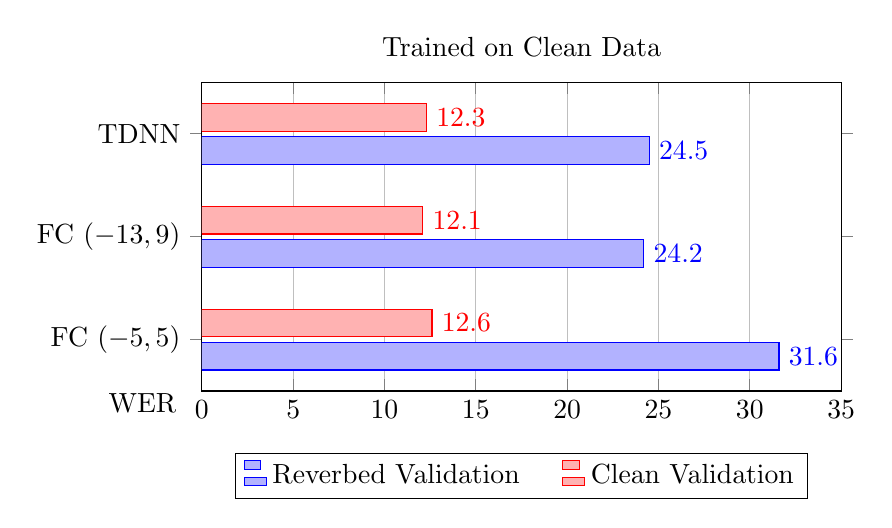
\begin{tikzpicture}
\begin{axis}[
title=Trained on Clean Data,
xbar,xmajorgrids=true,
width=0.8\linewidth,height=5.5cm, enlarge y limits=0.25,
xmin=0,xmax=35,xlabel={WER},xlabel style={
	at={(ticklabel cs:0)},
	anchor=north east,
	yshift=0.56 cm, xshift=-0.2cm
},
symbolic y coords={FC \text{$(-5,5)$}, FC \text{$(-13,9)$}, TDNN},
ytick=data,nodes near coords, nodes near coords align={horizontal},
legend style={at={(0.5,-0.2)},
	anchor=north,legend columns=2}
]
\addplot coordinates {(31.6,FC \text{$(-5,5)$}) (24.2,FC \text{$(-13,9)$}) (24.5,TDNN)};
\addlegendentry{Reverbed Validation \quad \quad}
\addplot coordinates {(12.6,FC \text{$(-5,5)$}) (12.1,FC \text{$(-13,9)$}) (12.3,TDNN)};
\addlegendentry{Clean Validation}
\end{axis}
\end{tikzpicture}
\end{minipage}
\\ \\ \\ 
\begin{minipage}{\linewidth}
\centering
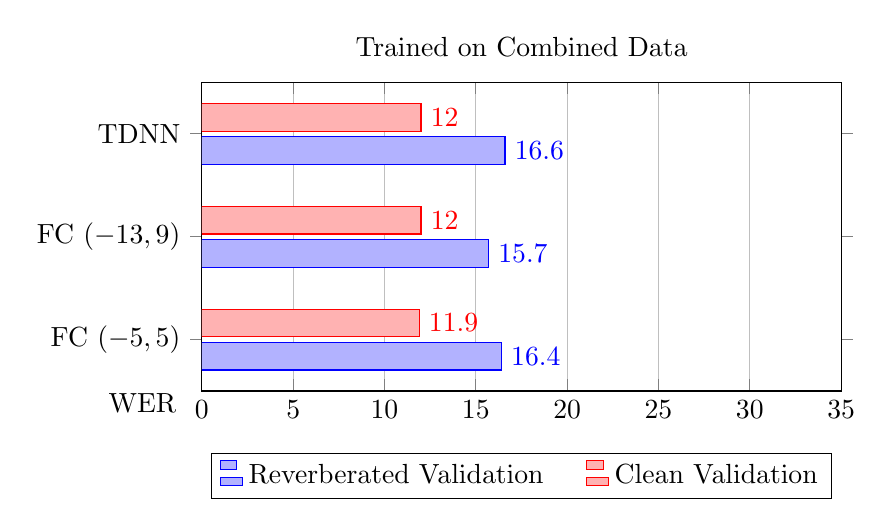
\begin{tikzpicture}
	\begin{axis}[
	title=Trained on Combined Data,
	xbar,xmajorgrids=true,
	width=0.8\linewidth,height=5.5cm, enlarge y limits=0.25,
	xmin=0,xmax=35,xlabel={WER}, xlabel style={
       at={(ticklabel cs:0)},
	   anchor=north east,
	   yshift=0.56 cm, xshift=-0.2cm
	},
	symbolic y coords={FC \text{$(-5,5)$}, FC \text{$(-13,9)$}, TDNN},
	ytick=data,nodes near coords, nodes near coords align={horizontal},
	legend style={at={(0.5,-0.2)},
		anchor=north,legend columns=2}
	]
	\addplot coordinates {(16.4,FC \text{$(-5,5)$}) (15.7,FC \text{$(-13,9)$}) (16.6,TDNN)};
	\addlegendentry{Reverberated Validation \quad \quad}
	\addplot coordinates {(11.9,FC \text{$(-5,5)$}) (12,FC \text{$(-13,9)$}) (12,TDNN)};
	\addlegendentry{Clean Validation}
	\end{axis}
	\end{tikzpicture}
	\captionof{figure}{Word Error Rate on the clean and reverberated validation dataset for models trained on clean and combined training data, respectively}
	\label{fig:final_validation}
\end{minipage} 
\end{minipage} 
\\ \\ \\
For models trained on reverberated data, the performance on reverberated validation is similar data for all three models. The same holds for clean validation data. The fully connected model with a large input context outperformed the other models on the reverberated validation set by a small margin. All models performed slightly better on clean validation data than the same model trained on clean data only, where the difference was most significant for the fully connected model with short input context. \\ \\
From this observations we conclude that data augmentation can be sufficient for improving acoustic model performance for reverberated audio. A larger input context can improve the robustness of the acoustic model in some cases. 
\iffalse
TODO: Describe how we generated reverbed data
TODO: Describe how we tested on reverbed data
TODO: Describe final architecture and results

This chapter should summarize and interpret the results. It should give a clear insight
about which methods did decrease the FER and WER on reverbed and unreverbed data, respectivley.
\fi
%% LaTeX2e class for student theses
%% sections/conclusion.tex
%% 
%% Karlsruhe Institute of Technology
%% Institute for Program Structures and Data Organization
%% Chair for Software Design and Quality (SDQ)
%%
%% Dr.-Ing. Erik Burger
%% burger@kit.edu
%%
%% Version 1.3.2, 2017-08-01

\chapter{Conclusion}
\label{ch:Conclusion}
During our evaluation in chapter \ref{ch:results} we found that our TDNN model did not yield a significant improvement over a fully connected model when trained on reverberated data. We also found that a fully connected model with the same input context was capable of slightly outperforming our TDNN model on the reverberated data validation set. This results are difficult to generalize to TDNNs as a whole for the following reasons: 
\begin{itemize}
	\item In chapter \ref{ch:tdnn_design}, we tuned our TDNN on clean data, with the assumption that a TDNN model that performs well on clean data also performs well on reverberated data. 
	\item The room impulse response normalization given in \ref{ch:results} might have been too aggressive, thus negating the advantage of TDNNs. In general, it is hard to measure the comprehensibleness of reverberated audio objectively.  
	\item In literature \cite{peddinti2015jhu} \cite{peddinti2015reverberation}, sMBR training criteria are used for TDNN acoustic model training. It might be worth to investigate this training procedure more closely.  
\end{itemize}
While the question whether TDNNs or fully connected networks are better for this specific problem is still unanswered, we provide several interesting insights that can improve speech recognition systems:
\begin{itemize}
	\item The modified L2 pooling nonlinearity introduced in section \ref{sec:tdnn_nonlin} performed better than L2 pooling combined with normalization.
	\item Augmented data can be used to boost the performance of acoustic models, even when only clean audio is of concern, as shown in chapter \ref{ch:results}.
	\item The calculation of priors from the network output, as shown in section \ref{sec:tdnn_prior}, given a randomly sampled subset of the training data, was shown to outperform priors which were calculated from the training data set. 
\end{itemize}
Overall, we were able to show that acoustic models can be made robust against reverberation, if they are trained using reverberated data as well.

%% --------------------
%% |   Bibliography   |
%% --------------------

%% Add entry to the table of contents for the bibliography
\printbibliography[heading=bibintoc]

%% ----------------
%% |   Appendix   |
%% ----------------
\appendix
%% LaTeX2e class for student theses
%% sections/apendix.tex
%% 
%% Karlsruhe Institute of Technology
%% Institute for Program Structures and Data Organization
%% Chair for Software Design and Quality (SDQ)
%%
%% Dr.-Ing. Erik Burger
%% burger@kit.edu
%%
%% Version 1.3.2, 2017-08-01


\chapter{Appendix}
\label{ch:appendix}
The appendix will contain information that might be useful for readers but 
does not fit anywhere else:
\begin{itemize}
  \item Practical pitfalls during training
  \item Implementation details
  \item If applicable, raw result data
\end{itemize}

\end{document}
